\documentclass[11pt]{article}
\usepackage[margin=1in]{geometry}
\usepackage{amsmath,amssymb,amsthm}
\usepackage{booktabs}
\usepackage{enumitem}
\usepackage[colorlinks=true,linkcolor=black,urlcolor=blue]{hyperref}
\usepackage{textcomp}
\usepackage{tikz}
\usetikzlibrary{arrows.meta,positioning,calc,decorations.pathreplacing}
\setlength{\parindent}{0pt}
\setlength{\parskip}{0.8em}

\newcommand{\code}[1]{\texttt{#1}}
\newtheorem{proposition}{Proposition}

\title{\vspace{-1.5em}Maximum-Flow Network Interdiction via QUBO Solvers\\
\large Problem summary, derivations, and research notes --- Network-Interdiction project}
\author{}
\date{}

\begin{document}
\sloppy
\maketitle
\vspace{-2em}

\textbf{What this is.} Part~I summarizes the problem the repository attacks, the three reformulations it uses, what the code actually implements and the experimental protocol behind the group's D-Wave runs, the derivations that say when the QUBO's ground state is the right answer (with proofs, and a check against the sample benchmark), the D-Wave results on three graph families, and the surrounding literature. Part~II holds the exploratory threads --- the original brainstorm on convex relaxations versus SA/QA, two concrete warm-start methods from the literature, and the divide-and-conquer / subgradient work in progress --- and ends by tying each thread to the specific result in Part~I it depends on, which yields an ordering for the open issues, and by mapping the CQT Year-4 proposal's commitments onto those issues (Section~\ref{sec:proposal}). Sources are the \code{Network-Interdiction} repository, the group's slide deck \code{S-T\_NIP.pptx} (16 slides; formulation, penalty argument, protocol, results, WIP), and the papers cited inline.

\tableofcontents

\part*{Part I --- Problem summary}

\section{The problem}

\textbf{Maximum-flow network interdiction (MFNIP).} Given a directed graph $G=(V,A)$ with source $s$, sink $t$, integer arc capacities $u_a > 0$, and an interdiction budget $B$, an attacker removes at most $B$ arcs so as to minimize the maximum $s$--$t$ flow that survives:
\begin{equation}
\label{eq:bilevel}
\min_{x \in \{0,1\}^A,\ \sum_a x_a \le B}\ \ \max\text{-flow}\bigl(G \setminus \{a : x_a = 1\}\bigr).
\end{equation}
This is a bilevel (min--max) problem; Figure~\ref{fig:problem} shows it on the smallest benchmark instance. The repository's instances use unit interdiction cost per arc (so the budget is a cardinality), and integer capacities read from \code{testcases/*.flow}; the planar family comes from LEDA-generated maximal planar graphs with random arc orientations and random capacities (\code{leda\_to\_flow\_file}).

\begin{figure}[h]
\centering
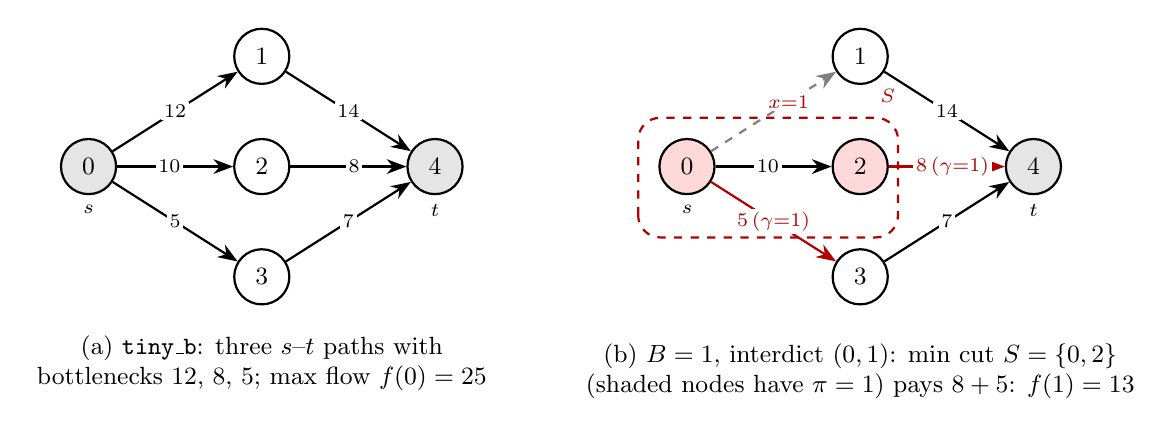
\begin{tikzpicture}[
  >={Stealth[length=2.5mm]},
  node/.style={circle,draw,thick,minimum size=7mm,inner sep=0pt,font=\small},
  term/.style={node,fill=black!10},
  arc/.style={->,thick},
  wt/.style={font=\scriptsize,fill=white,inner sep=1pt},
  cut/.style={->,thick,red!70!black},
  dead/.style={->,thick,dashed,gray},
  every label/.style={font=\scriptsize}
]
% ---------------- panel (a): original network ----------------
\begin{scope}
  \node[term,label=below:{$s$}] (s) at (0,0) {0};
  \node[node] (a) at (2.2,1.4) {1};
  \node[node] (b) at (2.2,0)   {2};
  \node[node] (c) at (2.2,-1.4){3};
  \node[term,label=below:{$t$}] (t) at (4.4,0) {4};
  \draw[arc] (s) -- node[wt,pos=0.5] {12} (a);
  \draw[arc] (a) -- node[wt,pos=0.5] {14} (t);
  \draw[arc] (s) -- node[wt,pos=0.45] {10} (b);
  \draw[arc] (b) -- node[wt,pos=0.55] {8} (t);
  \draw[arc] (s) -- node[wt,pos=0.5] {5} (c);
  \draw[arc] (c) -- node[wt,pos=0.5] {7} (t);
  \node[align=center,font=\small] at (2.2,-2.5) {(a) \code{tiny\_b}: three $s$--$t$ paths with\\bottlenecks $12,\,8,\,5$; max flow $f(0)=25$};
\end{scope}
% ---------------- panel (b): after interdiction ----------------
\begin{scope}[xshift=7.6cm]
  \node[term,fill=red!15,label=below:{$s$}] (s) at (0,0) {0};
  \node[node] (a) at (2.2,1.4) {1};
  \node[node,fill=red!15] (b) at (2.2,0)   {2};
  \node[node] (c) at (2.2,-1.4){3};
  \node[term,label=below:{$t$}] (t) at (4.4,0) {4};
  % source side S = {0,2}
  \draw[red!70!black,dashed,thick,rounded corners=8pt] (-0.62,-0.9) rectangle (2.68,0.62);
  \node[font=\scriptsize,text=red!70!black] at (2.55,0.9) {$S$};
  % interdicted arc: crosses the cut but is not paid for
  \draw[dead] (s) -- node[wt,pos=0.62,text=red!70!black] {$x{=}1$} (a);
  \draw[arc] (a) -- node[wt,pos=0.5] {14} (t);
  \draw[arc] (s) -- node[wt,pos=0.45] {10} (b);
  % cut arcs
  \draw[cut] (b) -- node[wt,pos=0.55,text=red!70!black] {$8$\,($\gamma{=}1$)} (t);
  \draw[cut] (s) -- node[wt,pos=0.5,text=red!70!black] {$5$\,($\gamma{=}1$)} (c);
  \draw[arc] (c) -- node[wt,pos=0.5] {7} (t);
  \node[align=center,font=\small] at (2.2,-2.6) {(b) $B=1$, interdict $(0,1)$: min cut $S=\{0,2\}$\\(shaded nodes have $\pi=1$) pays $8+5$: $f(1)=13$};
\end{scope}
\end{tikzpicture}
\caption{The problem on the smallest three-path benchmark instance. (a) The attacker sees the network and its capacities; the max flow is the sum of the three path bottlenecks. (b) With budget $B=1$ the best single arc to remove is $(0,1)$, the bottleneck of the widest path; the surviving max flow is $13$, certified by the cut $S=\{0,2\}$ whose crossing arcs $(2,4)$ and $(0,3)$ carry $8+5$. In the MILP \eqref{eq:milp} (whose $\pi,\gamma$ are the max-flow LP's dual variables, Section~\ref{sec:duals}), $x_a=1$ marks the removed arc, $\pi_i=1$ marks the source side $S$, and $\gamma_a=1$ marks the crossing arcs. The removed arc $(0,1)$ also crosses the cut (so the constraint $\pi_0-\pi_1\le\gamma_{(0,1)}$ forces $\gamma_{(0,1)}=1$), but its capacity is not paid for: that is the bilinear term $u_a(1-x_a)\gamma_a$ vanishing at $x_a=1$. Node $1$ sits on the sink side because putting it in $S$ would make $(1,4)$ cross at cost $14$.}
\label{fig:problem}
\end{figure}

\textbf{Complexity.} MFNIP is NP-hard in general (Wood 1993; Phillips 1993). Two facts worth keeping in view because they shape what ``hard instance'' can mean for issue \#1:
\begin{itemize}[leftmargin=1.5em]
\item Phillips (1993) gives a pseudo-polynomial algorithm on \emph{planar} graphs via the planar dual. The repository's benchmark family is planar. That does not make them easy for a general-purpose MILP solver, but it does mean ``hard for Gurobi'' on this family is a statement about the monolithic formulation, not about intrinsic hardness --- worth confirming against Phillips' construction before building the benchmark set on planar instances alone.
\item The LP relaxation of the standard single-level formulation below has a large integrality gap (Altner, Ergun \& Uhan 2010, who also give valid inequalities), so the root bound is weak; Chestnut \& Zenklusen (2017) give a 2-approximation and matching hardness-of-approximation results. The weak root bound is the specific reason branch-and-bound trees on this problem grow the way they do.
\end{itemize}

\section{Reformulations}

\subsection{Single-level MILP by dualizing the inner max flow (Wood 1993)}

Fix $x$. The surviving max flow equals the minimum $s$--$t$ cut in $G$ with capacities $u_a(1-x_a)$, and the min-cut LP
\[
\min_{\gamma \ge 0,\ \pi}\ \sum_{a=(i,j)} u_a (1-x_a)\,\gamma_a
\quad \text{s.t.}\quad \gamma_a \ge \pi_i - \pi_j\ \ \forall a,\qquad \pi_s - \pi_t \ge 1
\]
has a totally unimodular constraint matrix, so it has an integral optimum with $\pi \in \{0,1\}^V$ marking the source side of the cut and $\gamma_a \in \{0,1\}$ marking cut arcs. Substituting this for the inner problem turns \eqref{eq:bilevel} into a single-level 0--1 program:
\begin{equation}
\label{eq:milp}
\min_{x,\gamma,\pi \in \{0,1\}}\ \sum_a u_a(1-x_a)\gamma_a
\quad\text{s.t.}\quad \pi_i - \pi_j - \gamma_a \le 0\ \ \forall a=(i,j),\qquad \pi_t - \pi_s \le -1,\qquad \sum_a x_a \le B .
\end{equation}
This is exactly \code{solve\_nip\_gurobi}. The objective is bilinear in $(x,\gamma)$; Wood linearizes it with $\gamma_a \ge \pi_i - \pi_j - x_a$ (an interdicted arc need not be paid for even if it crosses the cut), whereas the repository keeps the product and lets Gurobi linearize binary products internally. Both are exact.

\subsection{What the duals are}
\label{sec:duals}

The $\pi$ and $\gamma$ variables are not modelling conveniences: they are the dual variables of the max-flow linear program, and that is the reason \eqref{eq:milp} is exact. Written out, for a fixed interdiction $x$ the inner problem is
\[
\begin{array}{r@{\quad}l@{\qquad}l}
\text{(max-flow)} & \displaystyle \max_{\phi \ge 0}\ \sum_{a \in \delta^{+}(s)} \phi_a
  & \\[1ex]
\text{s.t.} & \displaystyle \sum_{a \in \delta^{+}(i)} \phi_a - \sum_{a \in \delta^{-}(i)} \phi_a = 0 & \forall i \in V\setminus\{s,t\} \quad \text{(dual variable } \pi_i\text{)} \\[1ex]
 & \phi_a \le u_a (1-x_a) & \forall a \in A \quad \text{(dual variable } \gamma_a\text{)}
\end{array}
\]
with $\phi_a$ the flow on arc $a$. Attaching a multiplier to each constraint --- a node potential $\pi_i$ to conservation at $i$, a price $\gamma_a \ge 0$ to the capacity of $a$ --- and taking the LP dual gives
\[
\text{(min-cut)}\qquad \min_{\gamma \ge 0,\ \pi}\ \sum_a u_a(1-x_a)\,\gamma_a
\quad\text{s.t.}\quad \gamma_a \ge \pi_i - \pi_j\ \ \forall a=(i,j),\qquad \pi_s - \pi_t \ge 1 ,
\]
which is the LP in the previous subsection. Strong LP duality says its optimal value \emph{equals} the max flow, for every $x$; that is the max-flow/min-cut theorem, obtained here as a corollary of duality rather than as a separate combinatorial fact.

\emph{Reading the duals.} Fix $\pi_s = 1, \pi_t = 0$ (only the difference matters). An optimal dual can always be taken with $\pi_i \in \{0,1\}$, so $\pi$ is the indicator of a set $S \ni s$, $t \notin S$: the source side of a cut. The constraint $\gamma_a \ge \pi_i - \pi_j$ then forces $\gamma_a = 1$ on exactly the arcs that leave $S$, and $\gamma_a = 0$ is optimal everywhere else, so the objective is the capacity of the cut $(S, V\setminus S)$. Figure~\ref{fig:problem}(b) is this reading drawn out. Complementary slackness supplies the economic interpretation: $\gamma_a > 0$ only on arcs that are saturated ($\phi_a = u_a(1-x_a)$), and flow is positive only on arcs with $\gamma_a = \pi_i - \pi_j$ --- the arcs on which the potential drop is exactly the price. Node potentials that increase by one across the cut and are flat elsewhere are the certificate that no more flow can pass.

\emph{Why integrality is free.} The dual constraint matrix is the transpose of a network matrix, hence totally unimodular; every vertex of the dual polytope is $0/1$. That is what lets \eqref{eq:milp} declare $\pi,\gamma$ binary without changing the optimum, and it is the observation, made in Part~II, that the only fractionality in the LP relaxation of \eqref{eq:milp} comes from the budget row.

\emph{A second, different dual.} The multiplier $\lambda$ in \eqref{eq:lagr} is a \emph{Lagrangian} dual variable for the budget constraint of the outer problem, not an LP dual: the inner variables stay integer, so only weak duality holds, $L(\lambda) \le$ opt for all $\lambda \ge 0$, and the best bound $\max_\lambda L(\lambda)$ can sit strictly below the optimum. Proposition~\ref{prop:lambda} is precisely the statement of when that gap is zero. The naming in the code follows this split: the ``dual penalty'' $\beta$ enforces the min-cut (LP-dual) constraints inside the QUBO, and the ``cardinality penalty'' $\lambda$ \emph{is} the Lagrangian dual variable, used as a fixed penalty coefficient rather than optimized.

\subsection{Lagrangian relaxation of the budget}

Move the budget into the objective with multiplier $\lambda \ge 0$:
\begin{equation}
\label{eq:lagr}
L(\lambda) = \min_{x,\gamma,\pi}\ \sum_a u_a(1-x_a)\gamma_a + \lambda\Bigl(\sum_a x_a - B\Bigr)\quad\text{s.t. the cut constraints of \eqref{eq:milp}}.
\end{equation}
This is what \code{solve\_nip\_gurobi\_relaxation} solves repeatedly, bisecting on $\lambda$ until the minimizer uses at most $B$ arcs. It is a \emph{Lagrangian} relaxation, not an LP relaxation: the variables stay binary, and $L(\lambda) \le$ the optimum of \eqref{eq:milp} for every $\lambda \ge 0$ (weak duality). Section~\ref{sec:derivations} says exactly when some $\lambda$ recovers the optimum.

\subsection{Penalized QUBO (\code{nip\_to\_qubo})}
\label{sec:qubo}

The QUBO route keeps the Lagrangian treatment of the budget and additionally penalizes the cut constraints. Write $\pi_s \equiv 1$, $\pi_t \equiv 0$ (substituted, so the $\pi_t - \pi_s \le -1$ constraint is enforced exactly and those two qubits do not exist). The constraint $\pi_i - \pi_j - \gamma_a \le 0$ on binaries is violated in exactly one pattern, $(\pi_i,\pi_j,\gamma_a) = (1,0,0)$, so its natural penalty is the cubic indicator
\[
\mathbb{1}[\text{violated}] = \pi_i (1-\pi_j)(1-\gamma_a) = \pi_i - \pi_i\pi_j - \pi_i\gamma_a + \pi_i\pi_j\gamma_a .
\]
A QUBO cannot carry the cubic monomial, so \code{nip\_to\_qubo} introduces one auxiliary binary $w_a$ per arc and uses
\begin{equation}
\label{eq:Pa}
P_a(\pi_i,\pi_j,\gamma_a,w_a) = \pi_i - \pi_i\pi_j - \pi_i\gamma_a + w_a(\pi_i + \pi_j + \gamma_a - 1) + (\pi_i\pi_j + \pi_i\gamma_a + \pi_j\gamma_a) - (\pi_i + \pi_j + \gamma_a),
\end{equation}
which simplifies to $P_a = \pi_j\gamma_a - \pi_j - \gamma_a + w_a(\pi_i+\pi_j+\gamma_a-1)$. The full Hamiltonian, with coefficients $(\lambda, \beta)$ passed as \code{(cardinality\_penalty\_coeff, dual\_penalty\_coeff)} and $\beta = \lambda + 1$ wherever the repository calls it, is
\begin{equation}
\label{eq:H}
H(x,\gamma,\pi,w) = \sum_a u_a(1-x_a)\gamma_a + \lambda\Bigl(\sum_a x_a - B\Bigr) + \beta \sum_a P_a ,
\end{equation}
over $n = 3|A| + |V| - 2$ binary variables. Note the cardinality term is \emph{linear} in $\sum x_a$, not the squared $(\sum x_a - B)^2$ one usually sees --- it is a Lagrangian term, and that single fact explains most of the penalty-tuning behaviour observed in the repository (Section~\ref{sec:derivations}).

\section{What the repository implements}
\label{sec:impl}

\begin{itemize}[leftmargin=1.5em]
\item \textbf{Exact:} \eqref{eq:milp} in Gurobi (\code{solve\_nip\_gurobi}); the penalized model \eqref{eq:H} also in Gurobi as an exact check of a given $(\lambda,\beta)$ (\code{gurobi\_verify\_parameters}); Lagrangian bisection \eqref{eq:lagr} (\code{solve\_nip\_gurobi\_relaxation}). All need a Gurobi license beyond trial size.
\item \textbf{Heuristic:} build \eqref{eq:H} with PyQUBO, sample it with simulated annealing (\code{dwave-neal}, 2500 reads) or a D-Wave Advantage QPU (\code{EmbeddingComposite}, 2500 reads, $50\,\mu$s anneal, followed by steepest descent), decode the 20 lowest-energy samples, evaluate each decoded $x$ by an \emph{actual} max-flow computation rather than by its energy, and repair each to exactly $B$ arcs with a greedy add/remove pass (\code{improve\_dwave\_solution}). Reported: best surviving flow among budget-feasible samples, best after greedy repair, and best energy.
\item \textbf{Unsupported:} the iterative $\lambda$-search variants that shelled out to a Julia QUBO builder (\code{nip\_cubic.jl}, issue \#5) raise \code{NotImplementedError}.
\item \textbf{Benchmark pipeline (PR \#13):} \code{run\_benchmark.py} produces one CSV row per (instance, $B$, $\lambda$) with exact reference columns from Gurobi or, for tiny instances, from exhaustive search plus \code{dimod.ExactSolver}; \code{network\_interdiction\_plot.py} draws flow-reduction and energy ratios against the exact optimum.
\end{itemize}

\textbf{Experimental protocol behind the D-Wave runs} (slide 7 of \code{S-T\_NIP.pptx}; the code paths above are its implementation):
\begin{itemize}[leftmargin=1.5em]
\item \emph{Instances.} Three random families: maximal planar graphs (embedded with the linear-time algorithm of Stamm-Wilbrandt 1993; the \code{testcases/*.u} LEDA files), 2D $k$-nearest-neighbour graphs, and Erd\H{o}s--R\'enyi graphs. Each undirected edge is oriented at random, then reverse arcs are added until the digraph is strongly connected; capacities are random integers. Budgets $B$ from $4$ to $12$.
\item \emph{Penalty coefficients.} $\lambda_1$ (our $\lambda$) by binary search over $[\min_a u_a, \max_a u_a]$; $\lambda_2$ (our $\beta$) set to $\lambda_1 + 1$. Because QPU time was budgeted, the search is run with classical simulated annealing as the inner solver, and the QPU is queried once, at the final $\lambda_1$.
\item \emph{Sampling and decoding.} 2500 samples; the 20 with the lowest QUBO energy are decoded and their surviving flow computed exactly; the best is reported. Each of the 20 is also greedily post-processed to exactly $B$ arcs: if over budget, remove the interdicted arcs with the least impact one at a time; if under, add the arc with the most impact one at a time (\code{improve\_dwave\_solution}).
\end{itemize}

\section{Derivations and results}
\label{sec:derivations}

Everything below is about when the ground state of \eqref{eq:H} is the optimum of \eqref{eq:milp}. Let $f(k)$ denote the best surviving flow using at most $k$ interdicted arcs ($f$ is nonincreasing, $f(0)$ is the max flow), and $u_{\max} = \max_a u_a$.

\begin{proposition}[The auxiliary variable quadratizes the cubic penalty exactly]
\label{prop:quad}
For every $(\pi_i,\pi_j,\gamma_a) \in \{0,1\}^3$,
\[
\min_{w_a \in \{0,1\}} P_a(\pi_i,\pi_j,\gamma_a,w_a) = \pi_i(1-\pi_j)(1-\gamma_a) - 1 ,
\]
and $P_a \ge \pi_i(1-\pi_j)(1-\gamma_a) - 1$ for either value of $w_a$.
\end{proposition}
\begin{proof}
Using the simplified form $P_a = \pi_j\gamma_a - \pi_j - \gamma_a + w_a(\pi_i+\pi_j+\gamma_a-1)$: the $w_a$-free part equals $-1$ unless $(\pi_j,\gamma_a)=(0,0)$, where it is $0$. The coefficient of $w_a$ is $\pi_i+\pi_j+\gamma_a-1 \in \{-1,0,1,2\}$, so $\min_{w_a} w_a(\cdot) = -1$ when the coefficient is $-1$, i.e.\ when $(\pi_i,\pi_j,\gamma_a)=(0,0,0)$, and $0$ otherwise. Checking the eight cases: the minimum is $0$ at $(1,0,0)$ --- the violating pattern --- and $-1$ everywhere else, which is the claimed identity. The lower bound holds because a minimum over $w_a$ is at most either value.
\end{proof}

Slide 6 of \code{S-T\_NIP.pptx} states this quadratization as an equality, $\min a\,xyz = \min_w a\{w(x+y+z-1) + xy+yz+xz-(x+y+z)\}$; it holds up to the additive constant $-a$, which is harmless for the minimizer and is where the offset below comes from.

Two consequences. First, the ground-state energy of \eqref{eq:H} carries a constant offset of $-\beta|A|$, which is why every \code{Opt\_QUBO} in the sample CSV is negative; energies are comparable across $\lambda$ only after removing it. Second, since $w_a$ enters no other term, minimizing $H$ over $w$ is exact, and one may reason about $H$ with $\beta\sum_a \mathbb{1}[\text{violated}_a]$ in place of $\beta \sum_a P_a$.

\begin{proposition}[Dual penalty]
\label{prop:beta}
If $\beta > \lambda$, every ground state of $H$ violates no cut constraint. The same holds if $\beta > u_{\max}$, for every fixed $x$ separately. In either case a ground state's energy is the true surviving max flow $\text{max-flow}(G\setminus\{a : x_a=1\})$ plus $\lambda(\sum_a x_a - B) - \beta|A|$.
\end{proposition}
\begin{proof}
Take any configuration with a violated arc $a=(i,j)$: $\pi_i=1,\pi_j=0,\gamma_a=0$. A violation is an arc that leaves the cut side $S$ without being paid for --- an interdiction that dodges the $\lambda$ charge. Make it honest: set $\gamma_a=1$ and $x_a=1$. The cut term $u_a(1-x_a)\gamma_a$ is $0$ before and after, the $\beta$ charge disappears, and the $\lambda$ charge appears only if $x_a$ was $0$; the net change is at most $\lambda - \beta < 0$. (If $x_a$ was already $1$, setting $\gamma_a = 1$ alone saves $\beta$ at no cost.) So under $\beta>\lambda$ every violating configuration is strictly dominated and no ground state has one. The $u_{\max}$ variant repairs the violation without touching $x$: setting $\gamma_a=1$ costs at most $u_a(1-x_a)\le u_{\max}$ and saves $\beta$. A violation-free $(\gamma,\pi)$ with $\pi_s=1,\pi_t=0$ is an $s$--$t$ cut of cost $\sum_{a\in\text{cut}}u_a(1-x_a)$; minimizing over cuts gives the min cut, i.e.\ the max flow on the surviving graph.
\end{proof}

The first condition is the one that matters: it is the argument on the ``proof for penalty coefficients'' slide of \code{S-T\_NIP.pptx} ($\lambda_2 \ge \lambda_1$ in the slides' notation, strict here for uniqueness), and it is exactly why the repository's choice $\beta = \lambda + 1$ is safe --- on every instance, independent of the capacities. On the sample rows $\beta$ is below $u_{\max}$ (e.g.\ $\beta=7$ against $u_{\max}=10$ on \code{tiny\_a}), so the second, capacity-based condition is not what is protecting those runs; the first is. The practical consequence is that the dual penalty is not a tuning problem at all: only $\lambda$ is.

\begin{proposition}[Valid window for the linear cardinality penalty]
\label{prop:lambda}
Assume $\beta$ satisfies Proposition~\ref{prop:beta}. The ground state of $H$ interdicts exactly $B$ arcs and attains $f(B)$ if and only if
\begin{equation}
\label{eq:window}
\max_{k > B} \frac{f(B) - f(k)}{k - B}\ \ <\ \ \lambda\ \ <\ \ \min_{k < B} \frac{f(k) - f(B)}{B - k},
\end{equation}
with non-strict inequalities giving ties. In particular a valid $\lambda$ exists if and only if $B$ is a vertex of the lower convex envelope of $k \mapsto f(k)$.
\end{proposition}
\begin{proof}
By Proposition~\ref{prop:beta}, after minimizing over $(\gamma,\pi,w)$ the energy of a configuration with $k$ interdicted arcs is at least $f(k) + \lambda(k-B) - \beta|A|$, with equality for the best $k$-arc set. So the ground state minimizes $g(k) = f(k) + \lambda k$ over $k$, and $k=B$ is the unique minimizer exactly when $f(B)+\lambda B < f(k)+\lambda k$ for all $k \ne B$. Rearranging for $k<B$ and $k>B$ separately gives the two sides of \eqref{eq:window}. The set of $k$ minimizing $f(k)+\lambda k$ for some $\lambda \ge 0$ is precisely the set of vertices of the lower convex envelope of $f$ (a supporting line of slope $-\lambda$ touches $f$ at $k$), which is the existence statement.
\end{proof}

The slides state a different range, $\lambda_1 \in (\min_a u_a, \max_a u_a)$, with an argument that adding or removing an interdicted arc changes the objective by $u_a$. That is the step that does not hold: interdicting an arc changes the surviving flow by its \emph{marginal} effect on the min cut, which is at most $u_a$ and is $0$ for an arc on no minimum cut. So the slide range is neither necessary nor sufficient. It coincides with \eqref{eq:window} on \code{tiny\_a} and is a strict superset on the other sample instances --- on \code{tiny\_b} with $B=1$ it admits $\lambda = 6$, for which $g(k) = f(k)+6k$ takes the values $25, 19, 17, 18$ at $k=0,1,2,3$, so the ground state interdicts two arcs and overshoots the budget. The bisection the slides describe (and \code{solve\_nip\_gurobi\_relaxation} implements) still lands inside the true window in practice, because it searches for the largest $\lambda$ at which the minimizer respects the budget, which is the upper end of \eqref{eq:window} whenever that window is non-empty; it just cannot tell when the window is empty.

This is the mechanism behind the ``too-large $\lambda$ makes the annealer interdict nothing'' behaviour noted in the test suite and behind the narrow windows found when the sample CSV was generated: a large $\lambda$ makes $g$ increasing so $k=0$ wins, a small $\lambda$ makes $k$ overshoot $B$, and if $f$ is not convex at $B$ no $\lambda$ works at all --- the standard Lagrangian duality gap for integer programs, showing up here as ``no penalty coefficient exists.'' Table~\ref{tab:windows} checks \eqref{eq:window} against the windows found empirically by sweeping $\lambda$ with \code{dimod.ExactSolver} on the six sample rows.

\begin{table}[h]
\centering
\small
\begin{tabular}{llllll}
\toprule
instance & $B$ & $f(0),f(1),f(2),f(3)$ & window \eqref{eq:window} & sweep hits ($\lambda$ step $0.5$) & $\lambda$ used \\
\midrule
\code{tiny\_a} & 1 & 15, 5, 0, 0 & $(5, 10)$ & $5.5, 6, \dots, 10$ & 6.0 \\
\code{tiny\_b} & 1 & 25, 13, 5, 0 & $(8, 12)$ & $8.5, 9, 9.5, \dots$ & 9.0 \\
\code{tiny\_b} & 2 & 25, 13, 5, 0 & $(5, 8)$ & $5.5, 6, 6.5, \dots$ & 6.0 \\
\code{tiny\_c} & 1 & 11, 4, 0, 0 & $(4, 7)$ & $4^{*}, 4.5, 5, \dots$ & 4.5 \\
\code{tiny\_d} & 1 & 22, 13, 6, 0 & $(7, 9)$ & $7.5, 8, 8.5$ & 8.0 \\
\code{tiny\_d} & 2 & 22, 13, 6, 0 & $(6, 7)$ & $6^{*}, 6.5, 7^{*}$ & 6.5 \\
\bottomrule
\end{tabular}
\caption{Predicted valid $\lambda$ window versus the values at which the exact QUBO ground state was observed to decode to an optimal $B$-arc interdiction. Starred entries sit on a window boundary, where the ground state is degenerate and the solver happened to return the right member of the tie. Every observed hit lies in the predicted window and every predicted interior point that was tried was a hit.}
\label{tab:windows}
\end{table}

\subsection{Results}
\label{sec:results}

\textbf{In the repository.} The only committed results are the sample benchmark: on the six tiny rows, simulated annealing (2500 reads) reaches the exact ground-state energy and the exact optimal flow both before and after greedy repair, so every plotted ratio is $1.0$. That demonstrates the pipeline, not performance --- at $14$--$22$ variables SA is effectively exhaustive.

\textbf{D-Wave results in the slide deck.} The runs the plotting script was written for exist as figures in \code{S-T\_NIP.pptx} (slides 8--10), one per graph family, though the CSVs behind them were never checked in. Each figure reports, per instance and budget, the flow reduction achieved relative to the Gurobi optimum ($1.0$ = optimal) for raw QA and SA and for their greedy-repaired versions; a missing raw bar means none of the 20 best samples was budget-feasible. The $x$-axis label is the QUBO variable count $|V| + 3|A|$ (the planar sizes $914, 1389, 2339$ are the $50$-, $75$- and $125$-node \code{testcases} instances). Table~\ref{tab:dwave} is read off those figures, so values are approximate to about $\pm 0.01$.

\begin{table}[h]
\centering
\small
\begin{tabular}{llcccc}
\toprule
family & QUBO vars ($B$) & raw QA & raw SA & QA-greedy & SA-greedy \\
\midrule
planar & 914 (5, 6, 8, 10) & $0.87$--$0.92$ & $0.84$--$0.93$ & $1.0$ & $1.0$ \\
       & 1389 (5, 8, 10)   & $0.60$--$0.73$ & --, --, $0.82$ & $1.0$ & $1.0$ \\
       & 2339 (6, 10)      & --, --         & $0.16$, --     & $1.0$ & $1.0$ \\
\midrule
Erd\H{o}s--R\'enyi & 1124 (5, 6, 8) & $0.89$--$0.95$ & $0.91$--$0.93$ & $1.0$ & $1.0$ \\
       & 1438 (7, 8, 10)   & $0.78$--$0.97$ & $0.89$--$1.0$  & $1.0, 1.0, 0.99$ & $1.0, 1.0, 0.99$ \\
       & 2370 (8, 10, 12)  & $0.70$--$0.86$ & $0.85$--$0.95$ & $1.0, 1.0, 0.97$ & $1.0, 1.0, 0.97$ \\
\midrule
2D $k$-NN & 1070 (4, 5, 6) & $0.37$, --, $0.47$ & --, --, -- & $1.0$ & $1.0$ \\
       & 1845 (6, 7, 8)    & --, --, $0.86$ & $0.81$, $0.79$, $0.86$ & $0.95, 0.94, 0.93$ & $0.95, 0.94, 0.93$ \\
       & 2398 (6, 7, 8)    & $0.52$--$0.90$ & $0.66$--$0.90$ & $0.90, 0.90, 0.94$ & $0.90, 0.90, 0.94$ \\
\bottomrule
\end{tabular}
\caption{Flow reduction relative to the Gurobi optimum on the D-Wave Advantage QPU (QA) and simulated annealing (SA), from slides 8--10 of \code{S-T\_NIP.pptx}. A dash means no budget-feasible sample among the 20 lowest-energy ones (the plots draw these as zero-height bars). Greedy columns are after the repair pass of Section~\ref{sec:impl}.}
\label{tab:dwave}
\end{table}

Four things the table says, which the per-family slides do not say together:
\begin{enumerate}[leftmargin=1.5em]
\item \emph{Raw annealer output degrades with size and is often infeasible.} At $\sim 900$--$1100$ variables raw QA and SA sit at $0.85$--$0.95$ of optimal; by $\sim 2300$ variables raw QA frequently produces no budget-feasible sample in its best 20, and on the $k$-NN family SA is infeasible on all three smallest instances. This is the linear budget penalty doing what Proposition~\ref{prop:lambda} says it does: $\lambda$ trades off against the objective rather than enforcing the budget, and low-energy samples land on either side of $B$.
\item \emph{Greedy repair is carrying the result.} On planar and Erd\H{o}s--R\'enyi graphs the repaired solutions are optimal in all but two instances (the ER $1438(10)$ and $2370(12)$ rows, at $0.99$ and $0.97$), including every case where the raw sample was infeasible or far from optimal. QA-greedy and SA-greedy are indistinguishable everywhere. Slide 12 supplies the likely reason: on these random families the optimal interdiction set consisted of arcs incident to $s$ or $t$, which a greedy ``remove the highest-impact arc'' pass finds without help. The experiment that separates the annealer's contribution from the repair's has not been run: greedy from a random or empty $x$, on the same instances.
\item \emph{The $k$-NN family is the one with signal.} It is the only family where greedy repair fails to reach the optimum ($0.90$--$0.95$ on the six larger instances), so it is the only family in this deck on which a better sampler, a better penalty, or a warm start could visibly improve the reported number. It is also, not coincidentally, the family whose raw feasibility is worst.
\item \emph{The QPU and SA are equivalent here.} No row separates QA from SA after repair, and raw QA is more often infeasible than raw SA at the largest sizes (consistent with embedding overhead on the Advantage topology at $\sim 2300$ logical variables). There is no quantum-advantage claim to be made from this data, and the deck does not make one.
\end{enumerate}

The deck's motivating example (slides 1--2: a four-node network, remove two arcs, max flow $25 \to 5$, ``an $80\%$ reduction'') is the same picture as Figure~\ref{fig:problem}; as drawn on the slide, the three arcs leaving $s$ have capacities $6+11+5=22$, so one capacity label there is stale relative to the stated $25$ and is worth fixing before the deck is reused.

\section{Existing work}

\textbf{Classical interdiction.} Wood (1993), \emph{Deterministic network interdiction}, Math.\ Comput.\ Modelling 17(2) --- NP-hardness, the dualized formulation \eqref{eq:milp}, and the linearization. Phillips (1993), \emph{The network inhibition problem}, STOC --- hardness in general, pseudo-polynomial algorithm for planar graphs. Israeli \& Wood (2002), \emph{Shortest-path network interdiction}, Networks 40(2) --- Benders decomposition for interdiction, the template for keeping the flow subproblem separate. Cormican, Morton \& Wood (1998), \emph{Stochastic network interdiction}, Oper.\ Res.\ 46(2). Altner, Ergun \& Uhan (2010), \emph{The maximum flow network interdiction problem: valid inequalities, integrality gaps, and approximability}, Oper.\ Res.\ Lett.\ 38(1). Chestnut \& Zenklusen (2017), \emph{Hardness and approximation for network flow interdiction}, Networks 69(4). Smith \& Song (2020), \emph{A survey of network interdiction models and algorithms}, Eur.\ J.\ Oper.\ Res.\ 283(3) --- the survey to start from.

\textbf{QUBO / annealing machinery.} Lucas (2014), \emph{Ising formulations of many NP problems}, Front.\ Phys.\ 2 --- the standard penalty encodings, including the squared cardinality penalty this repository does \emph{not} use. Glover, Kochenberger \& Du (2019), \emph{Quantum bridge analytics I: a tutorial on formulating and using QUBO models}, 4OR 17. Boros \& Hammer (2002), \emph{Pseudo-Boolean optimization}, Discrete Appl.\ Math.\ 123, and Ishikawa (2011), \emph{Transformation of general binary MRF minimization to the first-order case}, IEEE TPAMI 33(6) --- quadratization of higher-order terms, of which Proposition~\ref{prop:quad} is one instance. Hen \& Spedalieri (2016), \emph{Quantum annealing for constrained optimization}, Phys.\ Rev.\ Applied 5 --- constraint-preserving (fixed Hamming weight) drivers, the annealing side of issue \#3. Hadfield et al.\ (2019), \emph{From the QAOA to a quantum alternating operator ansatz}, Algorithms 12(2) --- the gate-model side of the same idea.

\textbf{Warm starts.} Egger, Mare\v{c}ek \& Woerner (2021); He et al.\ / Shaydulin (2026); Cain et al.\ (2022); Tate et al.\ (2023) --- detailed in Part II.

\textbf{What is missing.} I am not aware of a prior QUBO/annealing treatment of MFNIP specifically, and did not find one in the searches behind this note; that is a statement about the search, not the literature, and a proper check is a cheap first task. The repository's own QUBO construction --- Lagrangian budget term, cubic dual penalty quadratized through $w$ --- has no written derivation anywhere; Section~\ref{sec:derivations} is the first.

\part*{Part II --- Exploratory research threads}

Three threads follow. The first is the original brainstorm on whether SA/QA can use the convex relaxation the way branch-and-bound does; the second is what the warm-start literature actually prescribes; the third is the divide-and-conquer decomposition and subgradient penalty tuning marked work-in-progress in the slide deck. Section~\ref{sec:tie} then ties each thread back to the derivations in Part~I and to the open issues.

\section{Convex relaxations vs.\ SA/QA heuristics --- the original brainstorm}

The question that started this note: branch-and-bound gets its power from a convex relaxation; SA and QA don't use one --- why not, and could they? A couple of the premises needed a small correction before the ``why not'' makes sense.

\subsection*{Is it purely discrete?}

Yes --- every decision variable in the repo's formulations ($x$, $\gamma$, $\pi$, and the auxiliary $w$) is binary. Edge weights are fixed data, not decisions. There's no continuous decision variable anywhere; this is a 0-1 program, not a mixed-integer program with a meaningful continuous part.

\subsection*{What B\&B is actually doing (and a wrinkle worth knowing)}

At each node, Gurobi solves the LP relaxation (integrality dropped, $x \in [0,1]$) --- that's convex, gives a valid bound, and branching + cutting planes progressively shrink the gap between that relaxation and the true integer hull. So yes, ``convexify, bound, prune'' is the right mental model.

One wrinkle: this problem's objective isn't linear to begin with. \code{nip\_to\_qubo} and \code{gurobi\_verify\_parameters} have bilinear terms $(1-x)\gamma$ and, in the dual-linking term, a genuinely cubic term $\pi_u \pi_v \gamma$. For binary variables these are \emph{exactly} linearizable (McCormick/RLT: a product of binaries is itself binary, so $z = a\,b\,c$ can be captured exactly, not just approximated, with a few linear constraints --- that's what the \code{w} variable in \code{gurobi\_verify\_parameters} is doing). So what Gurobi is really solving is the LP relaxation of an exactly linearized reformulation, not a relaxation of the polynomial form directly.

\subsection*{The ``strongly convex $\Rightarrow$ local min = global min'' intuition --- where it applies and where it doesn't}

That argument is about a continuous, differentiable objective. The LP relaxation here is convex but not strongly convex (it's linear), and its optimum being ``the'' optimum isn't because gradients vanish --- it's because LP optima sit at polytope vertices and simplex/interior-point methods find the global one for free (convexity $\Rightarrow$ no spurious local optima to get stuck at).

The catch: the LP relaxation's optimum is a \emph{different problem's} optimum, not this problem's, and it only coincides with the true 0-1 optimum when the relaxation happens to be integral. Here's the interesting bit specific to this codebase: the \emph{inner} max-flow/min-cut LP is integral automatically --- network flow constraint matrices are totally unimodular, which is exactly why plain \code{nx.maximum\_flow} never needs integrality constraints. The fractionality --- and the NP-hardness --- comes entirely from bolting the attacker's budget constraint ($\sum x \le B$) and the duality-linking terms onto that otherwise-integral flow polytope. So the relaxation is tight everywhere except where the actual decision variables live, which is a pretty precise way of stating why this is hard.

\subsection*{So why can't SA/QA just use the convex relaxation the way B\&B does?}

Two separate reasons, and one of them dissolves into something more interesting than ``can't.''

\begin{enumerate}[leftmargin=1.5em]
\item Mechanically, SA and QA aren't gradient-following --- they're stochastic search over discrete/spin configurations (bit-flips accepted/rejected via the Metropolis criterion, or quantum tunneling between basins). A relaxation's bound is only useful to something that does bounding-and-pruning (B\&B); it doesn't plug into an update rule that has no notion of ``prune this branch.''

\item But --- and this is the interesting part --- annealing already does something structurally identical to what's being asked for, just with a generic surrogate instead of an LP-informed one. SA's high-temperature regime smooths the energy landscape into something close to convex (this is literally ``deterministic annealing'' / graduated non-convexity in the continuous-optimization literature --- cooling is a homotopy from a smooth surface down to the true rugged one). QA does the quantum-mechanical version explicitly: it starts in the ground state of a trivial transverse-field Hamiltonian (unique ground state, no barriers --- the ``convex'' end of the homotopy) and adiabatically deforms it into the problem Hamiltonian (the true nonconvex Ising landscape), tracking the ground state the whole way if the schedule is slow enough relative to the minimum spectral gap. That \emph{is} ``tie the convex surrogate's solution back to the nonconvex problem's solution'' --- it's just using a problem-agnostic convex surrogate (equal superposition / infinite temperature) rather than one built from this problem's actual LP relaxation.
\end{enumerate}

That reframes the question into a real, open one: \textbf{can the generic surrogate be replaced by one informed by the LP relaxation?} Concretely, three ways to actually do this, increasing in effort:

\begin{enumerate}[leftmargin=1.5em]
\item \textbf{Cheap classical baseline} --- solve the LP relaxation once, round the fractional $x/\pi/\gamma$, then run the same greedy repair already sitting in \code{improve\_dwave\_solution} (currently only used to patch infeasible SA/QA samples) to project it onto the budget-feasible set. This costs one LP solve, no annealing at all, and gives a fast baseline to compare SA/QA against --- right now there's no ``how good is a dumb LP-round-and-repair'' data point in the plan.

\item \textbf{Bound accounting for free} --- solve the relaxation once, use its objective as a valid lower bound, and report the gap against whatever SA/QA/Gurobi returns. That's B\&B's bounding step without the tree --- a one-line addition that turns every SA/QA run into a run with a certified (or at least estimated) optimality gap instead of just a number.

\item \textbf{Warm-starting the annealer} --- use the LP relaxation's fractional solution to bias the initial state (QA) or bias fields/initial temperature schedule (SA), instead of starting from the generic uniform/high-$T$ surrogate. This is exactly what ``warm-start QAOA'' does in the literature, and it connects directly to the constraint-aware mixer issue (\#3): a mixer restricted to the fixed-Hamming-weight (budget-respecting) subspace is a way of baking the polytope's structure into the search dynamics rather than penalizing it.
\end{enumerate}

One more thing worth naming explicitly, since it falls straight out of the TU-network observation above: the classical OR literature on network interdiction doesn't usually solve the penalized single-level MILP the way this repo does --- it typically uses \textbf{Benders decomposition}, exploiting exactly the fact that the inner max-flow LP is integral (Israeli \& Wood's dualization is the same trick used here, but Benders keeps the flow/cut structure as a subproblem instead of flattening everything into one big linearized MILP with cubic terms). That's likely a stronger and faster classical baseline than what's currently in \code{network\_interdiction.py}, and it would sharpen issue \#1 too --- it would tell us whether the ``hard for Gurobi'' instances are hard for the monolithic MILP specifically, or hard for network interdiction in general (Benders included).

\section{Two concrete warm-start recipes from the literature --- and whether we can implement them}

Item 3 above waved at ``warm-start QAOA.'' Two specific papers prescribe two different ways to build the warm start, and the difference matters for what we could actually run here. Throughout, $Q$ is the QUBO matrix that \code{nip\_to\_qubo} already produces (as a \code{dimod} BQM), $n = 3E + V - 2$ is its variable count, and $\lambda$ keeps its meaning from the rest of the repo (the cardinality penalty coefficient) --- the regularization weight below is written $\mu$ to avoid the clash.

\subsection*{A. Egger, Mare\v{c}ek, Woerner --- relaxation-seeded warm start (Quantum 5, 479, 2021)}

\emph{Recipe.} Solve a continuous relaxation of the QUBO once and read off $c^* \in [0,1]^n$. Prepare the product state
\[
|\phi^*\rangle = \bigotimes_i \hat R_Y(\theta_i)\,|0\rangle, \qquad \theta_i = 2\arcsin\sqrt{c_i^*},
\]
so that measuring qubit $i$ gives $1$ with probability exactly $c_i^*$. Then replace the standard mixer $-\sum_i \hat X_i$ by a rotated single-qubit mixer whose ground state is $|\phi^*\rangle$:
\[
\hat H^{(\mathrm{ws})}_{M,i} =
\begin{pmatrix} 2c_i^* - 1 & -2\sqrt{c_i^*(1-c_i^*)} \\ -2\sqrt{c_i^*(1-c_i^*)} & 1 - 2c_i^* \end{pmatrix}
= -\sin\theta_i\,\hat X_i - \cos\theta_i\,\hat Z_i ,
\]
which is implemented per layer as $\hat R_Y(\theta_i)\hat R_Z(-2\beta_k)\hat R_Y(-\theta_i)$ --- no extra two-qubit gates over plain QAOA.

\emph{Why the regularizer.} If the relaxation returns $c_i^* \in \{0,1\}$, qubit $i$ starts in a $\hat Z$ eigenstate, and since the cost Hamiltonian is diagonal and the mixer is aligned with that state, nothing in the circuit ever moves it. That's a reachability failure whenever the relaxed and integer optima disagree on that bit. Their fix is to clip: pick $\varepsilon \in [0, 0.5]$ and set $\theta_i = 2\arcsin\sqrt{\varepsilon}$ when $c_i^* \le \varepsilon$, $2\arcsin\sqrt{1-\varepsilon}$ when $c_i^* \ge 1-\varepsilon$ (mixer adjusted to match). $\varepsilon = 0.5$ recovers standard QAOA exactly; their numerics use $\varepsilon = 0.25$. With $\varepsilon > 0$ the initial state overlaps every basis state, so the usual adiabatic argument for $p \to \infty$ convergence goes through.

\emph{What you get for free.} At depth $p = 0$, measuring $|\phi^*\rangle$ \emph{is} randomized rounding of the relaxation, so the algorithm inherits the classical guarantee (Goemans--Williamson's $0.878$ for MaxCut when the relaxation is the SDP). Every extra layer can only be optimized on top of that.

\emph{Which relaxation.} For MaxCut they use the GW SDP; for general QUBO the quadratic-program relaxation $\min_{x \in [0,1]^n} x^\top Q x$. That QP is convex only if $Q \succeq 0$, which ours is not --- but on binaries $x_i^2 = x_i$, so adding $\sum_i d_i (x_i^2 - x_i)$ to the objective changes nothing on $\{0,1\}^n$ and any $d_i \ge \sum_{j \ne i} |Q_{ij}|$ makes the shifted matrix PSD (Gershgorin). The result is a box-constrained convex QP that \code{scipy} L-BFGS-B solves without Gurobi.

\emph{Mapping onto NIP.} Two cautions specific to this repo:
\begin{itemize}[leftmargin=1.5em]
\item The obvious relaxation to reach for is the LP relaxation of the linearized MILP (the one with the $w$ variables in \code{gurobi\_verify\_parameters}). That is \emph{not} what \code{solve\_nip\_gurobi\_relaxation} computes --- that function is a Lagrangian bisection on $\lambda$ with the variables still binary, so it returns an integer $x$, i.e.\ a warm \emph{bitstring}. Seeding QAOA with a bitstring and the standard mixer is precisely the setting Cain et al.\ show gets stuck (arXiv:2207.05089): a good guess is a near-eigenstate of the cost, and the $\hat X$ mixer then makes almost no progress. So the Lagrangian output is usable only through the $\varepsilon$-clipped state and rotated mixer, never as a bare initial state.
\item By the TU observation earlier, the $\pi/\gamma/w$ block is determined by $x$ through a min-cut, so a relaxation is fractional essentially only on the $x$ coordinates. That is where $\varepsilon$ does its work; the rest of the qubits will sit near $\{0,1\}$ and be clipped to $\varepsilon$ regardless.
\end{itemize}

\subsection*{B. He, Apte, Augustino, Babakhani, Khan, Omanakuttan, Shaydulin --- regularized warm start (arXiv:2603.10191, 2026)}

\emph{Recipe.} No relaxation solve at all. Choose the product state directly by optimizing its Bernoulli parameters $p_i = \sin^2(\theta_i/2)$ against the \emph{mean-field energy plus a regularizer}:
\[
\min_{p \in [0,1]^n}\ \mathcal{L}_\mu(p) = \mathbb{E}_{x \sim p}\big[x^\top Q x\big] - 4\mu \sum_i p_i(1-p_i),
\qquad
\mathbb{E}_{x \sim p}\big[x^\top Q x\big] = \sum_i Q_{ii}\,p_i + \sum_{i<j} Q_{ij}\,p_i p_j .
\]
The expectation is closed-form under a product distribution (each term costs one nonzero of $Q$), so a gradient step is $O(\mathrm{nnz}(Q))$ and the whole thing is cheap at any size we care about. The regularizer is maximal at $p_i = \tfrac12$ and zero at a bitstring, so subtracting it pulls every qubit \emph{away} from the classical extremes: $\mu \to \infty$ gives $p \equiv \tfrac12$ (standard QAOA), $\mu \to 0$ gives a mean-field collapse onto a bitstring. The mixer is the same rotated family as A --- $\hat H_M(\theta) = \sum_i \sin\theta_i\,\hat X_i + \cos\theta_i\,\hat Z_i$ up to sign convention --- aligned so the optimized state is its ground state. They run it \emph{non-variationally}: $(\gamma, \beta)$ are fixed in advance by optimizing on local subgraphs of representative instances and then transferred, which is what lets them go to $N = 10{,}000$ at depth 6 with tensor networks and to 96 nodes on Quantinuum hardware.

\emph{Why it doesn't stall.} Their argument is the clean version of the reachability problem in A: if the initial product state is a bitstring, it is a common eigenstate of the cost Hamiltonian and of the aligned mixer, so the QAOA unitaries act on it only by a phase and the algorithm explores nothing. The regularizer makes that state unreachable by construction rather than by post-hoc clipping. For $D$-regular MaxCut they show $\mu > D/4$ makes $\mathcal L_\mu$ strictly convex with a unique minimizer (they nonetheless find $\mu = 0.6$ works best for 3-regular, below the guarantee). For our weighted, non-regular $Q$ the same Gershgorin argument gives the sufficient condition $\mu > \tfrac18 \max_i \sum_{j \ne i} |Q_{ij}|$ with $Q_{ij}$ the BQM's quadratic biases counted once per pair --- large for us, because the penalty terms with coefficient $\lambda$ sit in exactly those off-diagonals. Expect the useful $\mu$ to be well below that bound, as it was for them.

\emph{Scope.} Stated for any QUBO; the paper explicitly leaves constrained problems as future work. Our penalized QUBO qualifies as a QUBO, but note the regularizer and the cardinality penalty now compete inside $\mathcal L_\mu$: $\lambda$ wants the mean-field $x$ to have $\sum p_i \approx B$, $\mu$ wants every $p_i$ near $\tfrac12$. On an instance with $E \gg B$ those pull in opposite directions, so the $\mu$ window that neither collapses nor washes out the budget is another thing to sweep, on top of the $\lambda$ window issue \#2 is already about.

\subsection*{C. What is implementable now, with what is installed}

\begin{enumerate}[leftmargin=1.5em]
\item \textbf{The RWS product-state optimizer, today.} $\mathcal L_\mu$ and its gradient are a few dozen lines of \code{numpy} over the \code{dimod} BQM \code{nip\_to\_qubo} already returns; projected gradient descent on $[0,1]^n$. No Gurobi, no LP, no new dependency. Output: $p \in [0,1]^n$.

\item \textbf{Using $p$ without any gate-model machinery.} The annealer analogue of ``start in $|\phi^*\rangle$'' is ``start SA from bitstrings drawn from $p$'': \code{neal.SimulatedAnnealingSampler.sample} accepts \code{initial\_states}, and \code{solve\_qubo\_via\_dwave.py} already uses that argument for the steepest-descent pass. Sampling $2500$ initial states from $\mathrm{Bernoulli}(p)$ instead of uniformly is a one-line change in the \code{sa} path, keeps the regularizer's diversity (it does not collapse every read onto one guess), and is directly measurable against the sample benchmark by adding an \code{sa-ws} pass to \code{run\_benchmark.py}. On the QPU the analogue is reverse annealing (\code{initial\_state} + \code{anneal\_schedule} + \code{reinitialize\_state} on \code{DWaveSampler}) from a rounded $p$. Neither is QAOA, but both are the same idea on the stack we have, and either would tell us within an afternoon whether relaxation-informed starts move the SA/QA numbers at all.

\item \textbf{Actual WS-QAOA / RWS-QAOA needs a gate-model simulator}, which is not in \code{requirements.txt}. \code{qiskit-optimization} ships Egger's method as \code{WarmStartQAOAOptimizer} (with the $\varepsilon$ knob); RWS would be a custom initial state plus the rotated mixer on top of any QAOA implementation. Statevector simulation covers the $14$--$22$-qubit \code{tiny\_*} instances comfortably and nothing near \code{50.planarflow} ($n \approx 300$), so this is a tool for the mixer study in \#3, not for the scaling question in \#1. It is a dependency decision worth making deliberately.

\item \textbf{Egger's route additionally needs the relaxation.} The convexified QP above is the cheapest honest option (scipy, no license). The LP relaxation of the linearized MILP is the one with the OR-textbook meaning, but it needs an LP solver --- Gurobi when licensed, otherwise \code{scipy.optimize.linprog} (HiGHS) on a model we would have to build by hand since \code{gurobi\_verify\_parameters} builds it in \code{gurobipy} terms. Worth noting that these two relaxations are genuinely different objects: the QP relaxes the \emph{penalized} QUBO, so its fractional $c^*$ is partly shaped by $\lambda$ rather than by flow structure, whereas the MILP LP relaxation keeps the budget as a constraint. Comparing the warm starts they produce would itself be informative.

\item \textbf{The open design question is composition with constraint-preserving mixers.} Both warm-start mixers are products of single-qubit rotations and do not preserve Hamming weight; the fixed-$\sum x = B$ mixers from \#3 do, and are not products. Neither paper addresses combining the two (RWS names constrained problems as future work; Tate et al.'s custom-mixer line, arXiv:2112.11354, is also unconstrained). A warm start inside a constraint-preserving subspace would need the initial state to live in that subspace --- a Dicke-like state biased by $p$, not a product state --- and a mixer aligned to it. That is a research item, not an implementation item, and it is the one place where this thread and \#3 actually meet rather than merely sit next to each other.
\end{enumerate}

\emph{Sources.} Egger, Mare\v{c}ek, Woerner, ``Warm-starting quantum optimization,'' Quantum \textbf{5}, 479 (2021), \href{https://arxiv.org/abs/2009.10095}{arXiv:2009.10095}. He, Apte, Augustino, Babakhani, Khan, Omanakuttan, Shaydulin, ``Regularized warm-started quantum approximate optimization and conditions for surpassing classical solvers on the Max-Cut problem,'' \href{https://arxiv.org/abs/2603.10191}{arXiv:2603.10191} (2026). Cain, Farhi, Gutmann, Ranard, Tang, ``The QAOA gets stuck starting from a good guess,'' \href{https://arxiv.org/abs/2207.05089}{arXiv:2207.05089}. Tate, Moondra, Gard, Mohler, Gupta, ``Warm-started QAOA with custom mixers provably converges and computationally beats Goemans--Williamson's Max-Cut at low circuit depths,'' \href{https://arxiv.org/abs/2112.11354}{arXiv:2112.11354}.

\section{Divide and conquer, and subgradient tuning of $\lambda$ --- work in progress from the slides}
\label{sec:dnc}

Slides 11--12 of \code{S-T\_NIP.pptx} sketch two further directions. Both are recorded here as stated, with what Part~I adds to each.

\subsection*{Decomposition}

\emph{As proposed.} Partition the unweighted graph into contiguous pieces (METIS, or an edge separator); assign each arc to the piece of its tail, so separator arcs are owned by the piece their source lies in. Split the budget $B$ between pieces either in proportion to how many arcs of a global min cut each piece owns, or by estimating each piece's local max flow with super-source/super-sink nodes attached to its boundary vertices. Solve an NIP in each piece and combine. The current prototype keeps the whole graph and only restricts which arcs may be interdicted, which shrinks the classical search space but leaves the QUBO the same size --- the slide's own criticism --- and it floats contracting the other piece to a single node when solving one.

\emph{What Part~I adds.}
\begin{itemize}[leftmargin=1.5em]
\item The budget split is the entire difficulty, and it is a Lagrangian question. If piece $P$ gets budget $B_P$, the combined solution is optimal only if the marginal value of the last arc in each piece is equalized --- which is exactly the statement that one multiplier $\lambda$ serves all pieces. So a split by ratios of cut arcs or local flows is a heuristic for a common $\lambda$, and by Proposition~\ref{prop:lambda} a common $\lambda$ exists only if each piece's $f_P(k)$ is convex at its $B_P$. The decomposition and the penalty question are the same question.
\item Interdicting arcs in one piece changes the min cut and therefore the boundary flows of the other; local max flows computed once are stale after the first interdiction. Benders decomposition (Part~I, existing work) is the standard remedy: keep the pieces as flow subproblems and iterate cuts, rather than fixing the split up front.
\item Contraction is sound only if the contracted piece is not interdicted --- otherwise its internal capacity is not a constant. A contracted piece with budget $0$ can be replaced by its local max flow exactly; that is the case where contraction is a proof, not a heuristic.
\end{itemize}

\subsection*{Subgradient tuning of the cardinality penalty}

\emph{As proposed.} Drop the $\beta$ term (it is zero at any optimum, by Proposition~\ref{prop:beta}), write $\mathcal L(x,\lambda) = \sum_a u_a(1-x_a)\gamma_a + \lambda(\sum_a x_a - B)$, and maximize the dual $d(\lambda) = \inf_x \mathcal L(x,\lambda)$ by subgradient ascent: the subgradient at $\lambda$ is $\sum_a x^\lambda_a - B$, the excess of interdicted arcs over budget, where $x^\lambda$ minimizes $\mathcal L(\cdot,\lambda)$. The slide's stated problem: the minimizer $x^\lambda$ has to come from a heuristic QUBO solver.

\emph{What Part~I adds.}
\begin{itemize}[leftmargin=1.5em]
\item $d(\lambda) = \min_k f(k) + \lambda(k - B)$ is the lower convex envelope of $f$ evaluated at slope $-\lambda$, so $\max_\lambda d(\lambda)$ is the tightest Lagrangian bound and is attained on the window \eqref{eq:window} when that window is non-empty, and strictly below $f(B)$ otherwise. Subgradient ascent on $d$ is the principled version of the bisection on slide 7: same object, with a convergence theory and a certificate ($d(\lambda)$ is a valid lower bound at every iterate, heuristic or not).
\item The heuristic-argmin worry is real but asymmetric. A heuristic $\tilde x$ gives $\mathcal L(\tilde x,\lambda) \ge d(\lambda)$, so it \emph{overestimates} the bound (unsafe as a certificate) but its excess $\sum_a \tilde x_a - B$ is still a usable ascent direction in expectation. Using the exact decode (the max-flow evaluation the pipeline already does) rather than the QUBO energy for $\mathcal L(\tilde x,\lambda)$ removes the $\beta$ and offset noise from that estimate.
\item On the six sample rows, $d$ is computable exactly (Table~\ref{tab:windows} lists $f$), which makes them the right unit test for a subgradient implementation before it is pointed at an annealer.
\end{itemize}

\section{Tying the threads to the results}
\label{sec:tie}

Each exploratory idea above rests on something specific in Part~I. Making that dependence explicit is what turns a brainstorm into a work plan, because it says what has to be true --- or measured --- before the idea is worth an implementation.

\subsection*{The penalty structure comes first (issue \#2)}

Every heuristic result in this project is measured against the ground state of \eqref{eq:H}, and Propositions~\ref{prop:beta}--\ref{prop:lambda} say that ground state is the interdiction optimum only inside a $(\lambda,\beta)$ region that is instance-dependent, sometimes narrow, and sometimes empty. Three consequences for the rest of the plan:

\begin{itemize}[leftmargin=1.5em]
\item \textbf{The $\lambda$ window is computable, not searchable.} By \eqref{eq:window} it needs $f(k)$ for $k$ near $B$ --- on tiny instances by enumeration, on real ones by a handful of exact solves at neighbouring budgets, or by bounds on $f$ (the LP relaxation gives a lower bound on $f(k)$, the greedy repair an upper bound, and the window only needs the difference quotients). The current practice of sweeping $\lambda$ with an exact solver in the loop is doing by search what \eqref{eq:window} does in closed form. This is the concrete deliverable for \#2, and Table~\ref{tab:windows} is already its test.
\item \textbf{When the window is empty, no $\lambda$ can be ``derived.''} That is the case where $f$ is not convex at $B$. The fix is structural, not numerical: replace the linear term by the squared penalty $\lambda(\sum_a x_a - B)^2$ (Lucas 2014), whose valid range is a one-sided bound and always non-empty, at the cost of $O(|A|^2)$ new quadratic couplings; or keep the linear term and accept that the QUBO solves the Lagrangian dual, reporting $L(\lambda)$ as a bound rather than the answer. Which of these the project wants is a decision, and it should be made with the convexity of $f$ on the planar instances measured first.
\item \textbf{$\beta = \lambda + 1$ is already right; \#2 is about $\lambda$ alone.} Proposition~\ref{prop:beta} confirms the slide-deck argument that any $\beta > \lambda$ makes the ground state violation-free, independent of capacities, so the dual penalty needs no instance analysis. What does need one is the \emph{typical} width of the $\lambda$ window \eqref{eq:window} on the benchmark families --- how often it is empty, and how narrow it is when it is not --- since that is what decides whether a fixed or bisected $\lambda$ can work at all. The deterministic / almost-sure / average-case split used for the balanced-bisection penalty threshold in the sibling preconditioning project is the right template for that: worst case over capacities, the threshold under random capacities, and the per-instance window width in the bulk.
\end{itemize}

\subsection*{The relaxation threads (Part II, first thread) each rest on a different fact}

\begin{itemize}[leftmargin=1.5em]
\item \emph{LP-round-and-repair baseline} needs the LP relaxation of \eqref{eq:milp}, which the repository does not have (its ``relaxation'' function is the Lagrangian \eqref{eq:lagr}). Building it is one \code{scipy.optimize.linprog} model. Altner et al.'s integrality-gap result predicts that the rounded LP solution will often be poor --- which makes the baseline \emph{more} informative, not less: if SA/QA only match LP-round-and-repair, they are not extracting anything the LP did not already know.
\item \emph{Gap certificates} come from the same LP, or for free from $L(\lambda)$ in \eqref{eq:lagr}: by weak duality every Lagrangian value is a lower bound on the interdiction optimum, so the bisection the repository already runs produces certificates it currently throws away.
\item \emph{Benders decomposition} is the classical baseline that respects the TU structure (the cut subproblem is a max-flow, never a MILP). Its relevance to issue \#1 is the same as Phillips' planar result: both say the planar instances may be hard for the monolithic formulation and easy in fact. The benchmark set should be validated against Benders before anything is declared hard.
\end{itemize}

\subsection*{The warm-start thread (Part II, second thread) depends on the penalty structure twice}

\begin{itemize}[leftmargin=1.5em]
\item Both warm starts operate on the QUBO \eqref{eq:H}, so both inherit the $(\lambda,\beta)$ question: a warm start toward the ground state of a QUBO whose ground state is wrong is a warm start toward the wrong answer. Fix \#2 first, or run the warm-start experiments only on rows inside the window of Table~\ref{tab:windows}.
\item The regularized (RWS) objective $\mathcal L_\mu$ contains the Lagrangian term $\lambda\sum_a p_a$ through $\mathbb{E}[x^\top Q x]$, so $\lambda$ and $\mu$ interact: $\lambda$ pushes the mean-field $\sum_a p_a$ down toward $B$, $\mu$ pushes every $p_a$ toward $\tfrac12$, and with $|A| \gg B$ those are opposed. The window of useful $\mu$ is therefore a function of $\lambda$, and the sufficient uniqueness bound $\mu > \tfrac18 \max_i \sum_j |Q_{ij}|$ scales with $\beta$ through the dual-penalty couplings. This is a two-parameter sweep on the tiny rows before it is anything else.
\item The cheapest experiment in the whole document is the one that needs none of the gate-model machinery: RWS product state $\to$ Bernoulli($p$) initial states $\to$ \code{neal} with \code{initial\_states}. It tests the \emph{hypothesis} behind warm starts (that a relaxation-shaped start beats a uniform one on this landscape) on the solver the project already benchmarks, and it slots into \code{run\_benchmark.py} as one more pass. If it does nothing on the planar instances, the gate-model version is unlikely to either, and the project learns that for the price of an afternoon.
\item The composition of warm starts with constraint-preserving mixers (\#3) is where this thread and the penalty thread finally meet: a fixed-Hamming-weight mixer removes the need for the $\lambda$ term altogether (the budget is enforced by the subspace, so \eqref{eq:window} becomes moot), leaving only $\beta$. That is a strong argument for \#3 on its own, independent of warm starts, and it is the version of the problem in which a warm start would need to be a biased Dicke-type state rather than a product state --- an open construction.
\end{itemize}

\subsection*{The D-Wave results (Section~\ref{sec:results}) change what the benchmark question is}

\begin{itemize}[leftmargin=1.5em]
\item Table~\ref{tab:dwave} says the reported optimality comes from greedy repair on two of three families, and slide 12 says why (optimal arcs incident to $s$/$t$). Before any instance is called hard for issue \#1, run greedy repair from an empty and from a random $x$ on the same instances; whatever it reaches is the floor any annealer result has to beat. The deck's own next step --- real flow networks from the DIMACS max-flow collections instead of random families --- is the right one, and Phillips' planar result (Part~I) says the planar family should be dropped from the ``hard'' set regardless.
\item The $k$-NN family is where a method change could show: it is the only family with headroom after repair. It should be the primary target for the warm-start pass and for any change to the budget penalty.
\item Raw infeasibility at $\sim 2300$ variables is the linear-penalty tradeoff of Proposition~\ref{prop:lambda} made visible. The squared penalty would fix feasibility at the cost of density; a fixed-Hamming-weight mixer (\#3) would fix it at no density cost but only on gate-model hardware. This is the concrete evidence the linear-vs-squared decision in \#2 should be made on.
\end{itemize}

\subsection*{The decomposition thread (Section~\ref{sec:dnc}) is downstream of \#2, not parallel to it}

The budget split between pieces is a common-multiplier problem, so it inherits every property of the $\lambda$ window; and the subgradient method is the principled form of the bisection already in the code, with the sample rows as its exact unit test. The order is therefore: subgradient tuning of $\lambda$ on whole instances first (it is small, certifiable, and slots into \code{run\_benchmark.py}), decomposition after, and contraction only for zero-budget pieces where it is exact.

\subsection*{Ordering}

The dependencies above give an order that is not the order the issues were filed in (issue numbers as of Section~\ref{sec:proposal}):

\begin{enumerate}[leftmargin=1.5em]
\item Recover the CSVs behind slides 8--10 into \code{results/} so Table~\ref{tab:dwave} stops being read off a figure, and add the greedy-from-scratch baseline on the same instances (\#18, \#15).
\item Measure $f(k)$ near $B$ on the benchmark instances and compute the $\lambda$ window from \eqref{eq:window}; implement subgradient tuning of $\lambda$ with the sample rows as its unit test; decide linear vs.\ squared budget penalty on the raw-feasibility evidence in Table~\ref{tab:dwave} (\#2).
\item Add the LP relaxation and its two free by-products (LP-round-repair baseline, gap certificate), and a Benders baseline (\#15); replace the random families with real networks from the proposal's application domains and re-examine which instances are hard for what (\#1).
\item Run the \code{sa-ws} regularized-warm-start pass, on the $k$-NN family first; only if it moves the numbers, take on a gate-model QAOA dependency for the mixer study (\#3), which is also the prerequisite for parameter transfer (\#16) and the IBM path (\#17).
\item Decomposition (\#14) last, framed as a common-multiplier problem, with contraction restricted to zero-budget pieces; restore the QCI path (\#17) whenever the client code is located, since it is independent of the rest.
\end{enumerate}

\section{The CQT Year-4 proposal: commitments and the issues that carry them}
\label{sec:proposal}

The proposal \emph{Decomposition-Based Approaches for Practical Quantum Optimization} (Bernal, Pothen; CQT Year~4) makes four commitments that touch this repository. Table~\ref{tab:proposal} maps each to the issue that now tracks it; the ones numbered 14--18 were opened from this note, the comments on \#1 and \#2 were posted at the same time, and everything else is pre-existing.

\begin{table}[h]
\centering
\small
\begin{tabular}{p{0.42\textwidth}p{0.52\textwidth}}
\toprule
proposal text & where it lives \\
\midrule
\emph{Project description:} NIP formulated as a QUBO by dualize-and-combine then Lagrangian relaxation; ``only a small, dense submatrix''; on D-Wave with synthetic networks ``over 80\% optimal in small-to-mid instances, and greedy post-processing recovers optimal solutions in all instances.'' &
Formulation: Part~I, \S2--\S4 (the linear Lagrangian term is what keeps the QUBO sparse; Prop.~\ref{prop:lambda} is its price). Claim: \textbf{\#18} --- Table~\ref{tab:dwave} shows it holds for the planar family only; ER has two sub-optimal rows, $k$-NN six at $0.90$--$0.95$; raw feasibility fails at $\sim 2300$ variables. The CSVs behind the figures are to be recovered into \code{results/}. \\
\midrule
\emph{Milestone Q1:} ``further increase the sizes of network interdiction problems that can be solved on NISQ devices via decomposition-based refinement.'' &
\textbf{\#14} (new), built on the slide-deck design (\S\ref{sec:dnc}) with the common-multiplier analysis; \#4 keeps the scaling-axis inventory. \\
\midrule
\emph{Milestone Q1:} ``apply transfer parameter learning to increase scalability'' (the GAT parameter-transfer approach from the MIS work, proposal ref.~[5]). &
\textbf{\#16} (new), which depends on a QAOA existing first (\#3) and notes that RWS-QAOA (\S7) is the same idea with a regularized warm start; \#2 because transfer across $\lambda$ regimes transfers to the wrong Hamiltonian. \\
\midrule
\emph{Milestone Q3--4:} ``comparing decomposition approaches against classical methods.'' &
\textbf{\#15} (new): greedy-from-scratch, LP round-and-repair with its gap certificate, Lagrangian bound accounting, and Benders --- the four baselines Part~II's first thread and the tie-in called for; none existed as an issue. \\
\midrule
\emph{Milestone Q3--4:} ``test implementations on D-Wave, QCI, and IBM devices.'' &
\textbf{\#17} (new): the \code{qci} branch calls a \code{solve\_qubo\_via\_qci} module that is not in the repository (\code{NameError} if reached) and expects the Julia-era file format; there is no gate-model path for IBM at all until \#3/\#16 produce one. \\
\midrule
\emph{Industry/government need:} adversary interception, infectious disease control, power-system failure isolation. &
Comment on \textbf{\#1}: one real network per named domain; exclude instances whose optimal interdiction is incident to $s$/$t$ (slide~12); time Benders as well as the MILP before calling anything hard; drop the planar family from the hard set (Phillips 1993). \\
\midrule
--- (not in the proposal, but the derivations in \S\ref{sec:derivations} change the task) &
Comment on \textbf{\#2}: $\beta > \lambda$ suffices (no tuning); $\lambda$ has the exact two-sided window \eqref{eq:window}, sometimes empty, so the deliverable is the window computation, the linear-vs-squared decision, and subgradient tuning --- not a one-sided lower bound. \\
\bottomrule
\end{tabular}
\caption{Proposal commitments that concern the $s$--$t$ interdiction problem, and the issue or note section that now carries each. Issues \#14--\#18 were opened from this note on 2026-09-16.}
\label{tab:proposal}
\end{table}

Two things in the proposal text deserve a flag beyond the table. The results sentence is stronger than the data in the group's own slides, and it will be read by the site directors against whatever the Year-4 talk or poster shows; \#18 exists so that the next version of that sentence is by family. And the proposal's second milestone --- integer encodings for QUIO --- is not an $s$--$t$ interdiction item and has no issue here on purpose; if the budget variable or the capacities are ever encoded as integers rather than penalized binaries, that is where it would connect.

\bigskip
\noindent\textbf{Open question:} open issues for these --- (1) LP-round-repair baseline, (2) relaxation-based gap certificates for SA/QA/QAOA runs, (3) LP-informed warm-starting tied into the mixer work, (4) Benders decomposition as a stronger classical baseline, (5) a regularized-warm-start \code{sa-ws} pass in \code{run\_benchmark.py} as the cheap first experiment, (6) computing the $\lambda$ window from \eqref{eq:window} and subgradient tuning of $\lambda$ as the deliverable for \#2, (7) the greedy-from-scratch baseline and real-network instances that Table~\ref{tab:dwave} calls for, (8) decomposition as a common-multiplier problem --- (1)--(4) and (7)--(8) are now \#15, \#14, and the comments on \#1/\#2; (5)--(6) remain to be filed --- in the order of Section~\ref{sec:tie}, or keep brainstorming first?

\end{document}
